\documentclass[a4paper, oneside]{memoir}

\usepackage{pgfplots}
\usepackage{bookmark}
\usepackage{tocloft}
\usepackage{longtable}
\usepackage{booktabs}
\usepackage{array}
\usepackage{enumitem}
\usepackage{graphicx}
\usepackage{wrapfig}
\usepackage{listings}
\usepackage{amsmath}
\usepackage{bytefield}
\usepackage{siunitx}
\usepackage{hyperref}
\usepackage{bm}
\usepackage[backend=bibtex]{biblatex}
\addbibresource{PR1.bib}

\newcommand{\uvec}[1]{\boldsymbol{\hat{\textbf{#1}}}}

\setlength\cftchapterindent{\cftsectionindent}
\setlength\cftbeforechapterskip{0pt}
\setafterparaskip{1ex}
\setbeforeparaskip{-\beforeparaskip}
\renewcommand\cftchapterpagefont{\normalfont}
\setsecnumdepth{paragraph}

\renewcommand{\cftchapterleader}{\cftdotfill{\cftdotsep}}

\setlrmarginsandblock{1.25in}{1.25in}{*} 
\setulmarginsandblock{1.25in}{1.25in}{*} 
\checkandfixthelayout%

\renewcommand{\thesection}{\arabic{section}}
\renewcommand{\thefigure}{\arabic{figure}}
\renewcommand{\thetable}{\arabic{table}}

\lstset{language=C++,
                basicstyle=\ttfamily,
                keywordstyle=\color{blue}\ttfamily,
                stringstyle=\color{red}\ttfamily,
                commentstyle=\color{lightgreen}\ttfamily,
                morecomment=[l][\color{magenta}]{\#}
}

\newcommand*{\semester}[2]{Semester #1 -- #2} %chktex 8
\newcommand*{\student}[3]{&\text{#1} &\text{#2} &&\text{#3}} %chktex 8
\newcommand*{\titleAM}[4]%
{\begingroup
  \centering
  {\Huge Assessment Task #2:\\#3\par}\\[\baselineskip]
  {\Large HIVE AURC AVIONICS (Data Analytics and Verification)}\\[\baselineskip]
  {\small\scshape RMIT University}\par
  {\small\scshape #4}\par\vspace{0.5em}
  {\large Supervisor: #1}\par\vspace{0.5em}
  \endgroup}

\renewcommand{\tocheadstart}{}
\renewcommand{\aftertoctitle}{}
\renewcommand{\printtoctitle}[1]{}
\setcounter{tocdepth}{3}

\makeatletter
\DeclareRobustCommand{\cskippedwords}[2][2ex]{%
  \setlength{\units@wide}{\bf@bitwidth * \bits@wide}%
  \setlength{\units@high}{1pt * \ratio{\units@wide}{6.0pt}}%
  \setlength{\units@tall}{#1 + \units@high}%
  \edef\num@wide{\strip@pt\units@wide}%
  \edef\num@tall{\strip@pt\units@tall}%
  \edef\num@high{\strip@pt\units@high}%
  \begin{picture}(\num@wide,\num@tall)%
  \begin{tikzpicture}[overlay]
  \draw[fill=#2,fill opacity=0.2] 
    (0,-\bf@bitheight) -- (0,0) -- (0,\units@high) -- (\units@wide,0) -- +(0,-\bf@bitheight) -- cycle;
  \draw[fill=#2,fill opacity=0.2]
    (0,\units@high+#1+\bf@bitheight) -- ++(\units@wide,0) -- ++(0,-\bf@bitheight-\units@high) -- (0,\units@high+#1) -- cycle;
  \end{tikzpicture}%
  \end{picture}%
  \ifcounting@words
    \inc@bytefield@height{\unitlength * \real{\num@tall}}%
    \global\counting@wordsfalse
  \fi}
\makeatother

\usetikzlibrary{shapes.geometric, arrows}

\tikzstyle{start} = [rectangle, rounded corners, minimum width=3cm, minimum height=1cm, text centered, draw=black, fill=green!30]
\tikzstyle{stop} = [rectangle, rounded corners, minimum width=3cm, minimum height=1cm, text centered, draw=black, fill=red!50]
\tikzstyle{process} = [rectangle, minimum width=3cm, minimum height=1cm, text centered, draw=black, fill=orange!80, text=white]
\tikzstyle{decision} = [diamond, minimum width=3cm, minimum height=3cm, text centered, draw=black, fill=blue!50, text=white]
\tikzstyle{arrow} = [thick,->,>=stealth, draw=blue, text=blue]

\definecolor{bittersweet}{rgb}{1.0, 0.44, 0.37}
\definecolor{aquamarine}{rgb}{0.5, 1.0, 0.83}
\definecolor{lavender}{rgb}{0.9, 0.9, 0.98}
\definecolor{whitesmoke}{rgb}{0.96, 0.96, 0.96}
\definecolor{lightgreen}{RGB}{102,153,0}    %#669900

\lstset{language=C++,
        basicstyle=\ttfamily,
        keywordstyle=\color{blue}\ttfamily,
        stringstyle=\color{red}\ttfamily,
        commentstyle=\color{lightgreen}\ttfamily,
        morecomment=[l][\color{magenta}]{\#},
        backgroundcolor=\color{whitesmoke}
}

\renewcommand{\bibname}{References}
\newlist{questions}{enumerate}{2}
\setlist[questions,1]{label=RQ\arabic*.,ref=RQ\arabic*}
\setlist[questions,2]{label=(\alph*),ref=\thequestionsi(\alph*)}

\newcommand{\listquestionsname}{Research Questions}
\newlistof{listofquestions}{qu}{\listquestionsname}
\newcommand{\question}[1]{%
	\addcontentsline{qu}{question}{\protect\numberline{\thequestionsi}#1}\par
}
\makeatletter
\let\l@question\l@figure
\makeatother

\newcommand{\listequationsname}{List of Equations}
\newlistof{listofequations}{equ}{\listequationsname}
\newcommand{\myequation}[1]\\
    \student{Jeremy Timotius}{s3779178}{50\%}
  \end{align*}
  \addcontentsline{toc}{part}{Contents}
  \tableofcontents*
  \listofquestions \listofequations
  \clearpage
  \renewcommand{\abstractname}{Summary}

  \markboth{}{}
  
\addcontentsline{toc}{section}{\textbf{Summary}}
\begin{abstract}
  RMIT's high velocity rocket team (HIVE) this year is participating in the Australian Univercity Rocket Competition (AURC) under the 10,000ft category. As part of this competition HIVE proposed the completion of five rockets, given the name Aurora, with an iterative design approach working towards the fifth and final rocket that will fly as the competition entry vehicle. The Data Analytics and Verification team, a division of the avionics subsystem, was assembled for the purpose of producing the tools and implementation of both real-time and offline data processing systems that will run as a part of the rocket's avionics, as well as designing the verification routines to ensure proper testing procedure.
  \paragraph*{Key Milestones} 
  The following outlines a list of milestones reached throughout this project to date:
  \begin{itemize}
    \item Successful launch of Aurora I with data logged by avionics subsystem
    \item Design and implementation of dataframe specification
    \item Implementation and verification of designed state estimation through offline analysis 
      \begin{itemize}
        \item Attitude estimation through unit quaternion rotation
        \item Velocity estimation through Kalman Filter model
      \end{itemize}
    \item Design of A3 task structure for future implementation
  \end{itemize}\vspace{1em}

  Thus far the project has been largely successful, providing satisfactory results in preliminary testing and verification of developed systems. Some minor issues remain with current implementations, however these are majoritively insignificant to the overall functionality and key performance indicators. 

  Work now is posturing towards implementing these systems for the newly developed custom avionics hardware, with aim to have real time processing operational in the near future

  \paragraph*{Aurora I launch outcomes}
  The Aurora I rocket launched successfully on the 14th of April. Aurora I launched with a custom Avionics bay which included two commercial flight computers (Blue Raven) and a custom electronics system which contained an Arduino Nano, sensor suite and flash storage. From a Data analytics and verification perspective, the following outlines key outcomes and findings:
  \begin{itemize}
    \item Implementation: Custom firmware and libraries were created for the for Arduino Nano.  
    \item Data collection: Most data was successfully collected and stored by the system, however there was no available barometric data post-flight.
    \item Flash storage retrieval: Data was extracted from the on-board flash storage upon recovery.  
    \item Preliminary data validation: Initial comparison of sensor data with the Blue Raven recordings indicated general agreement in acceleration, velocity, and attitude trends. 
  \end{itemize}

  \paragraph*{Aurora II launch outcomes} 
  Aurora II launched a week prior to submission of this report, on Sunday the 26th of May. The rocket built for this launch was for the most part unchanged from Aurora I, with the original avionics system being re-flown with adjustments to ensure correct collection and storage of barometric data, in addition to ground communication hardware for preliminary telemetry testing from the Avionics, Ground Communications and Redundant Systems team. 

  As of the date of submission, data collected by the avionics system during this flight has yet to be retrieved. Once the data is available it will be applied for verification of the developed analysis tools and processing algorithms that will be further discussed later in the report.
\end{abstract}


\section{Introduction}
\subsection{Background and Significance}
The Aurora V rocket, a high-powered model rocket designed to reach an apogee of 10,000 feet, represents RMIT's entry in the 2024 Australian Universities Rocket Competition (AURC). To achieve a successful flight and meet the competition's requirements, real-time data collection, analysis, and verification is necessary. The Data Analytics and Verification team within the Avionics subsystem plays an important role in ensuring the rocket's performance, safety, and ultimately, the success of the mission. 

Aurora V will be the fifth and final competition ready rocket as it represents the culmination of the Aurora project as a whole. Throughout the semesters, previous iterations of the rocket (Aurora I to Aurora IV) will be developed and designed which will act a stepping stone towards the final design. With each iteration, the data gathered will feed into data analytics and verification processes in hopes to optimise algorithms and refine sensor configurations.  

The RMIT AURC team is multidisciplinary made up of five major sub systems including, Aerostructures, Avionics, Payload, Recovery and Aerobrakes totaling a team of 30 students. The Data analytics team is subset of the Avionics sub system and will provide insights into the rocket's flight dynamics, enabling real-time decision-making for critical systems like the airbrakes and switching over to failover systems. By analysing sensor data such as inertial measurements, barometric pressure, and temperature and through sensor fusion and filtering, an estimate of the rocket's position, velocity, and attitude can be measured. This information is mission critical for maintaining a stable trajectory towards the target apogee. Additionally, data verification and state estimations will be used to identify and mitigate potential errors or anomalies in the sensor readings, ensuring the reliability of the information used for flight control. 

The significance of this project extends beyond the immediate 2024 AURC competition as it will act as a resource for future RMIT model rockets. The development of data analytics and verification techniques for resource constrained embedded systems has a broader application in the aerospace industry and other fields where data analysis is critical. The work completed through this capstone will provide lessons and recommendations contributing to future work.  

\subsection{Problem Statement}
The primary challenge lies in designing and implementing firmware, data analytics and verification algorithms that can operate effectively within the limitations of the custom PCB board developed by the Aurora V's Avionics, Ground Communications and Redundant Systems team. This involves balancing the desire of captured sensor data and algorithms with the constraints of limited processing power, memory, and communication bandwidth. This subsystem’s primary objective is to design, test, and validate data analytics processes for the avionics, ground communications, redundant, electronic systems, and payload systems. 

\subsubsection{Project Deliverables}
Project deliverables and expected outcomes include:  
\begin{itemize}
  \item Data Capture and Logging Firmware Implementation: Defining sampling rates and intervals for data capture and establishing data logging and storing formats. 
  \item Real-Time Processing: Research and develop algorithms for sensor fusion to integrate data from multiple sensors. Implement filtering techniques to remove noise. Provide accurate state estimation for the airbrake control system. 
  \item Post-Processing: Perform statistical analysis to evaluate key performance metrics of avionics systems. Implement systems to detect deviations from expected behaviour when comparing raw sensor and fused data to the data captured by the blue raven. 
  \item Data Visualization: Develop tools for generating informative graphs and charts for data interpretation. Explore the possibility of creating simulations based on collected data. 
  \item Data Validation: Determine the validity of the captured sensor data.  
\end{itemize}

\subsubsection{Design/Research Questions}
\begin{questions}
  \item How accurate is the measured apogee to that provided by the Blue Raven (RMS error) \question{}
  \item How accurate are the calculated state values to that provided by the Blue Raven (RMS error) \question{}
  \item Do the selected hardware components remain functional under conditions expected during flight? \question{}
  \item What statistical analysis techniques will be employed to assess real time validity of data? \question{} \begin{questions}
    \item What communication protocols will be used to inform the redundant systems of detected errata?
    \item What metric(s) will the redundant systems use to elect which of primary and secondary sensors to sample?
  \end{questions}
\end{questions}

\subsubsection{Project Scope}
The Data analytics team is subset of the Avionics sub system and will operate within the project scope that encompasses the following activities: 
\begin{itemize}
  \item \textbf{Software Development}: Writing, testing, and optimizing firmware for data collection, logging, and real-time processing. Development post data visualization and analysis. 
  \item \textbf{Algorithm Design}: Researching and implementing algorithms for sensor fusion, filtering (Kalman filters), and state estimation. 
  \item \textbf{Testing and Validation}: Conducting ground tests and flight tests (Aurora I-V) to validate the performance and reliability of the data analytics and verification system. 
  \item \textbf{Iterative Refinement}: Continuously improving the system based on data and feedback from each launch, culminating in a competition-ready solution for Aurora V.
\end{itemize}

\paragraph{Limitations and Constraints}
The project focuses on the software and algorithmic aspects of data analytics and verification. Hardware design, development and initialisation of firmware fall under the Avionics Ground Communications and Redundant Systems team. 

The project timeline is subject to limitations and constraints, most notably the lead time required for procuring essential hardware components. This delay highlights the focus on software and algorithmic development while awaiting hardware delivery. During this waiting period, the team is using Nucleo-f439zi development board to prototype and test firmware and algorithms in a simulated environment. Additionally, sensor and integration verification tests are being designed to assess the performance and accuracy of firmware once the hardware becomes available. Furthermore, the team is actively analysing data captured during the Aurora I and II flights. This analysis aims to gain valuable insights into sensor behaviour, noise characteristics, and potential areas for algorithm optimisation. The findings from this analysis will directly inform the development of state estimation and Kalman filter implementations for Aurora III. 

While real-time data transmission is a goal, the primary focus is on ensuring reliable data logging for post-flight analysis and iterative improvement. This project scope is deliberately flexible to accommodate the iterative nature of rocket development. As new challenges and opportunities arise with each launch, the scope may be adjusted accordingly to ensure the successful completion of the project. 

\section{Literature Review}
During flight, the avionics subsystem is required to track various parameters of the rocket's state, both for the purposes of telemetry and for application in algorithms implemented by other on-board systems. In particular, it is imperative for the operation of the rocket's aerobrakes and recovery systems that accurate information concerning the upward velocity and altitude above ground are provided.

To determine these parameters, hardware sensors will be accessible for sampling both barometric and inertial data during flight. Importantly, accelerometers and gyroscopes provide information on the vehicle flight dynamics while a barometer samples pressure data that can be applied in calculation of vertical displacement. As the rocket's body axis during flight rotates off the global vertical, measurements from the accelerometer diverge from the true values. To account for this, attitude information that is calculated from the gyroscope is applied to rotate the data back to the global frame of reference.

\subsection{State Estimation}
A naive approach to state calculation would involve the numerical integration of sensor data to the required measurements. At a high level, MEMS (micro-electromechanical system) gyroscopes output axial data with units of degrees per second, and accelerometers provide acceleration measured in $\unit{G}$'s per second; Integrating these measurements, in theory, would result in the calculation of per-axis velocity and angular position. In reality, MEMS sensors are prone to drift from various noise sources~\cite{Diao2013, Pang2001} that results in error offsets which propagate with the integral summation. In addition, the mathematical constructs and operations that are utilised in these calculations can have a profound effect on the resulting output, particularly in the case of attitude determination from gyroscopic data.

Included amongst the most common representations of rotation in three dimensional space are Euler angles. These values are commonly referred to as \textit{roll}, \textit{pitch} and \textit{yaw}, and provide a convenient mapping of rotation to three spacial dimensions that correlate to the physical world, allowing intuitive understanding of the resulting metrics. While pleasant for human parsing, Euler angles are susceptible to difficulties that limit their application in attitude determination. In particular, the issues of rotational singularity and the strictness of their sequential nature complicates their implementation in the necessary calculations~\cite{Hemingway2018, Diebel2006}.

Alternatively, though complex in their mathematical structure, unit quaternions provide a more flexible representation of rotation that is not limited by these factors~\cite{Diebel2006}. Furthermore, quaternion rotations are easily compatible with Euler angles and can be integrated just as easily, allowing for more accurate instantaneous rotational calculations. It is also documented that the Blue Raven, to which the Aurora avionics system in large part emulates, makes use of quaternions for its attitude estimation~\cite{Adamson2023, Adamson2023timeseries}

Existing rocket designs such as Pioneer Rocketry's Skybreaker~\cite{Pioneer2016} and University of Calgary's Atlantis II~\cite{Atlantis2018} also make use of Kalman Filter implementations for apogee detection, fusing data both from barometric and inertial sensors to provide an estimate of the rocket's state during flight. These fiters attempt to provide an accurate estimation for noisy processes by using a model in combination with previous estimates to predict the future state of the process, correcting this prediction with measured data~\cite{Welch1995,kalman1960}. This process accounts for the process noise - deviation between the true state of the process and the state as described by the model - as well as the noise generated by the measurement of state values. A Kalman gain is computed to weight how much of the modeled and measured data should be accounted for in the new estimate, with an error covariance matrix tracking the uncertainty in the estimate.

Rockets built by university teams such as uORocketry and NTNU generally make use of positional data such as height or vertical displacement in combination with velocity measurements to control their aerobrake systems\cite{uORocketry, NTNU}. In order to accurately determine these parameters, errors accumulated within the measurement process may be eliminated through use of sensor fusion techniques. 

An example of how this may be applicable is in the altitude calculations. The most simple method of determining altitude would be to directly use the barometric pressure, however this is highly dependant on calibration at the launch site and susceptible to noise introduced from the sensor. An alternative would be to use integrated accelerometer data to obtain position, however the process of integrating itself is prone to drift due to time lag as well as flight angle offsets. A potential solution for these problems would be to combine the barometric altitude estimate together with positional calculations from the integrated accelerometer data, as described in a 2004 report by David Schulz\cite{kalman-apogee}. Accelerometer data can also be combined together with gyroscopic measurements from the IMU to rotate the inertial frame, allowing for pure vertical acceleration data to be integrated down to positional information. In all cases, some application of a Kalman Filter appears necessary.

\subsection{Real-Time Operating Systems}
The choice of an operating system (OS) for the avionics in Aurora V impacts system complexity, real-time performance, and resource utilisation. While bare-metal programming, where software directly interacts with hardware, offers simplicity and minimal overhead, it can become unmanageable as system complexity increases. As the number of processes increases, the harder it is to track timer and handle interrupts. This approach is suitable for resource constrained systems and has been employed in various amateur rocketry projects. 

The growing sophistication of model rocket avionics, as seen in projects like the Atlantis II, which employed FreeRTOS \cite{Atlantis2018}, has led to increased interest in Real-Time Operating Systems (RTOS) \cite{Di2018}. RTOS are specifically designed to handle real-time applications that require predictable timing behavior. An RTOS, such as FreeRTOS or VxWorks, provides features like prioritised thread scheduling, real-time clocks, and inter-process communication mechanisms that facilitate the development of reliable and responsive avionics software \cite{Dietrich2017}. For instance, the use of RTOS in embedded control systems like quadrotor flight controllers has demonstrated significant improvements in managing event latencies \cite{Di2018}. 

RTOS can abstract much of the complexity involved in timing and resource management, which allows developers to focus on application-specific logic. Additionally, the use of RTOS in the Atlantis II project highlights the need for a more structured software architecture as avionics systems incorporate multiple sensors, actuators, and communication interfaces.  

A Hybrid approaches may be considered which combine the benefits of both bare-metal and RTOS systems by integrating custom RTOS functionalities directly into hardware. This method reduces the overhead typically associated with full-blown RTOS, while still providing necessary real-time capabilities [3]. Such approaches have been shown to enhance performance by reducing interrupt lock times and memory usage, which is particularly beneficial in resource constrained environments such as the Aurora V.  

\section{Methodology and Engineering Design}
This section primarily outlines the engineering designs for Aurora I and Aurora III, detailing the progression of the avionics system across these developmental stages. Aurora II, a re-flight of Aurora I, utilised the same avionics board to provide further data for analysis and testing of derived algorithms, with no major changes made to its design. As these designs are implemented, testing and verification of hardware is to take place. 

\subsection{Aurora I }
Due to delays in hardware availability from vendors, the Aurora I avionics system resorted to “bare-bones" design, incorporating only essential components that were readily available. Although not ideal to the original Aurora I plan, the outcome still enabled the team to test fundamental functionalities including sensor data capture and writing data to flash storage. While limited in scope, the Aurora I design served as a stepping stone for subsequent iterations, providing initial data for post flight analysis. 

\subsubsection{Avionics Design Overview}
The Aurora I avionics system served as the initial prototype for data collection and recovery system testing. It consisted of two main components: 
\begin{itemize}
  \item Commercial Off-The-Shelf (COTS) Blue Raven Flight Computers: These flight computers were responsible for activating the recovery systems (drogue and main parachutes) and recording flight data for post-flight analysis. 
  \item Custom electronics board: This board, built on a perfboard, housed an Arduino Nano microcontroller, a sensor suite (accelerometer, barometer, gyroscope, magnetometer), and a flash storage module. The Arduino Nano controlled the sensors and data storage, while the flash module provided onboard data storage. 
\end{itemize}

\noindent The primary objectives of the Aurora I avionics system were to: 
\begin{itemize}
  \item Gain experience and understanding of the COTS Blue Raven flight computers. 
  \item Test various components of the avionics system, including battery types and sensor data collection. 
  \item Gather flight data for post processing and analysis
\end{itemize}

\subsubsection{Software Architecture}
The high-level flow chart provided under Appendix~\ref{apdx:A} depicts how the Aurora I avionics system captures and transmits data. The primary goal was to facilitate post-flight analysis and verification, aligning with the data collection intervals of the Blue Raven system ($\SI{500}{\hertz}$ high resolution and $\SI{50}{\hertz}$ low resolution). Due to timing constraints as a result of lesser performant hardware for Aurora I, the high resolution interval was elected to operate at $\SI{250}{\hertz}$ to ensure all processes have adequate time to complete. Data logging was initiated by a launch event detected when vertical acceleration exceeds a pre-defined threshold (5g at present). During flight, raw sensor data was stored onboard in flash memory.capabilities. 

\subparagraph{High Resolution Data Capture}

The high resolution interval ($\SI{250}{\hertz}$) focuses on data from an Inertial Measurement Unit (IMU), comprising accelerometer, gyroscope, and magnetometer sensors. This high sampling rate is used to accurately capture subtle changes in aircraft motion and orientation. Raw data from sensor registers is combined with headers into data frames, stored in a buffer, and then written to flash memory. 

\subparagraph{Low Resolution Data Capture and Transmission}

The low resolution interval ($\SI{50}{\hertz}$) reads data from a barometer (pressure and temperature sensor) to determine altitude. Similar to the high resolution process, raw data is framed and temporarily stored in a buffer before writing to flash. 

\subparagraph{Design Considerations and Implementation}

Alternative design approaches were considered, including a separate logging interval. However, the chosen design simplifies the system by consolidating flash writing and LoRa transmission into the low resolution interval. This streamlines data handling tasks while still meeting the core requirements. Although LoRa communications was included in the initial Aurora I software design, the hardware to support this was unavailable at the time due to delays in hardware delivery. As a result, testing for LoRa communications was organised to be implemented in Aurora II.  

\paragraph{Data Storage and Handling}

To support post-flight data processing, the sensor data is logged in a structured format using dataframes. This structured approach ensures that the host system can easily recognise and interpret the different types of data being read. 

\subparagraph{Data frame Structure}\label{sec:dataframe}

Each dataframe consists of a two-byte header and a payload. The header identifies the type of data recorded (e.g., high resolution, low resolution, or payload data), specifies the number of bytes in the payload, and includes a synchronisation byte for post-processing alignment. The payload contains the raw sensor data, organised in a specific order depending on the data type.  

To optimise storage efficiency and simplify implementation, the dataframes are stored in a \verb|uint8_t| buffer, where each byte represents an 8-bit unsigned integer. This choice is driven by the fact that some sensor data is 24-bits per sample and using 8-bit nibbles allows for efficient space utilization while maintaining simplicity. 

\begin{figure}[h]
  \begin{center}\hspace{4.5em}
  \begin{bytefield}[bitwidth=2em, endianness=big]{8}
    \bitheader{0,5,6,7}\\
    \begin{rightwordgroup}{Header}
      \bitbox{2}[bgcolor=bittersweet]{ID} 
      \bitbox{6}[bgcolor=aquamarine]{length}\\
      \wordbox{1}[bgcolor=aquamarine]{Sync} 
    \end{rightwordgroup}\\
    \begin{rightwordgroup}{Payload}
      \wordbox{1}{$D_0$[15:8]}\\
      \wordbox{1}{$D_0$[7:0]}\\
      \wordbox{1}{$D_1$[15:8]}\\
      \wordbox[lrt]{1}{}\\
      \cskippedwords{blue!20}\\
      \wordbox[lrb]{1}{}\\
      \wordbox{1}{$D_n$[7:0]}
    \end{rightwordgroup}
  \end{bytefield}
  \end{center}
  \caption{Dataframe structure for avionics}
  \label{fig:dataframe-structure}
\end{figure}

\subparagraph{Data Typing}

The data stored by the avionics system retains the raw structure as output by the onboard sensors, written as 8-bit unsigned blocks. This minimises storage requirements and avoids computational overhead during flight. Post-flight analysis can then convert this raw data into meaningful values by applying sensor-specific scaling factors and unit conversions. 

\begin{figure}[h]
  \begin{center}\hspace{4.5em}
  \begin{bytefield}[endianness=big]{16}
    \bitheader{0,15}\\
    \begin{rightwordgroup}{X-axis}
      \bitbox{8}[]{Upper nibble} 
      \bitbox{8}[]{Lower nibble} 
    \end{rightwordgroup}\\
    \begin{rightwordgroup}{Y-axis}
      \bitbox{8}[]{Upper nibble} 
      \bitbox{8}[]{Lower nibble} 
    \end{rightwordgroup}\\
    \begin{rightwordgroup}{Z-axis}
      \bitbox{8}[]{Upper nibble} 
      \bitbox{8}[]{Lower nibble} 
    \end{rightwordgroup}
  \end{bytefield}
  \end{center}
  \caption{Example structure for a single sensor payload}
  \label{fig:payload-structure}
\end{figure}

\paragraph{Synchronisation}

Synchronisation between high- and low resolution data, as well as with the Blue Raven data, is achieved using a "sync code”. Based off the Blue Raven data user guide, this code is a counter that increments every millisecond, wrapping around at 250. By including this sync code in the header of each dataframe, the system ensures that data from different sources can be accurately aligned and compared during post-flight analysis. As detailed above, this sync code is included as a full byte in the frame header, following the ID and frame length. This byte will be added into all saved data to ensure synchronisation consistency across all datasets

\subsection{Aurora III}
\subsubsection{Avionics Design Overview}
The Aurora III avionics system is designed to manage power, acquire flight and payload data, facilitate internal vehicle communication, and enable vehicle-to-ground communication. However, when compared to Aurora I and Aurora II, it also plays an additional role in supporting the Aerobrakes and Recovery subsystems by providing essential flight data which includes altitude and velocity. Ground communication through LoRa protocol will also be included within the systems, supporting live state estimates during flight. From a high-level perspective, the avionics system comprises two SRAD (Student-Research and Developed) flight computers, each equipped with its own sensor suite for redundancy. 

A block diagram illustrating the high-level design of the avionics system is shown in Figure~\ref{fig:avionics-block}

\begin{figure}[h]
  \begin{center}
    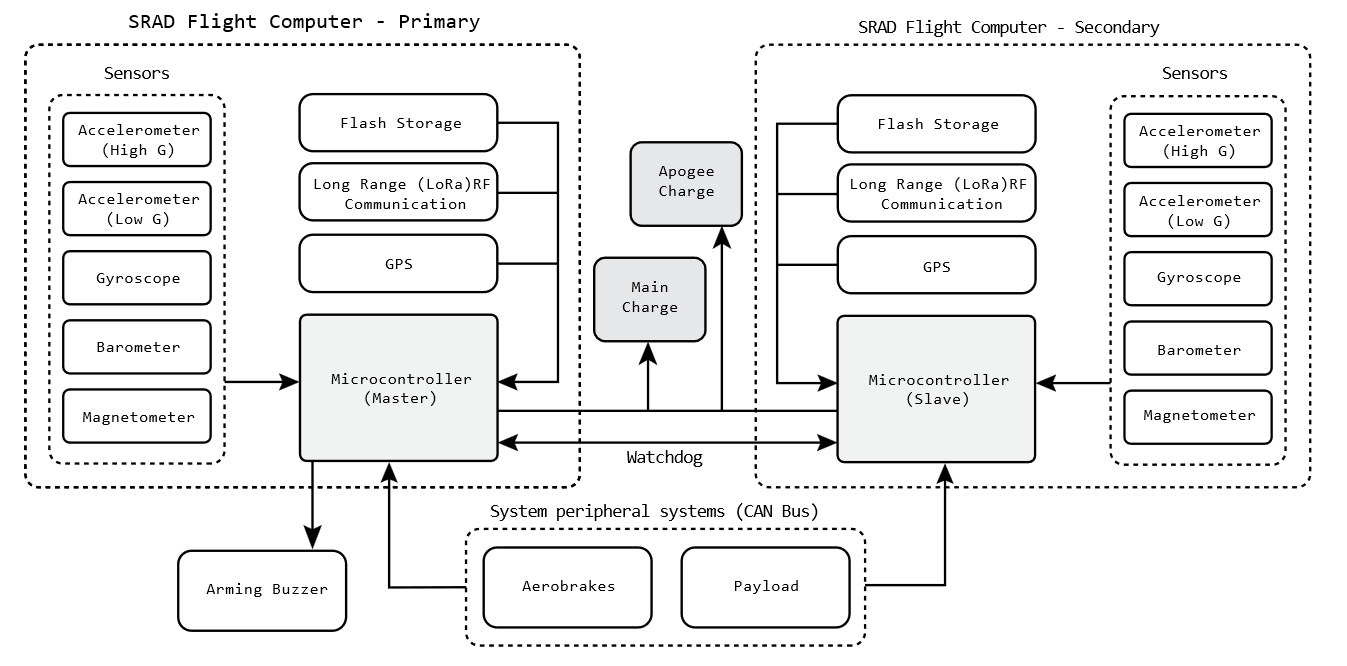
\includegraphics[width=0.95\textwidth]{./img/Section_4_1_A3_SRAD_design.jpg}
  \end{center}
  \caption{High-level block diagram provided by the Avionics, Ground Communications and Redundant Systems team}\label{fig:avionics-block}
\end{figure}


The system utilizes an STM32F439 microcontroller as its core processing unit. This microcontroller was chosen by the broader team for its familiarity, sufficient clock speed, ample I/O pins, and built-in SPI/I2C and CAN bus functionality. The addition of LoRa communication enables real-time data transmission to the ground station, enhancing monitoring and analysis capabilities. The system also incorporates the ability to receive and send data to the payload and aerobrakes subsystems via the CAN 2.0A protocol, facilitating integrated control and decision-making during flight. 

\subsubsection{Software Architecture}
The Aurora III avionics software will undergo a significant architectural shift with the introduction of a Real-Time Operating System (RTOS). This decision was driven by the increased complexity of the avionics system compared to Aurora I. The addition of communication with the Aerobrakes and Payload subsystems, along with the need for precise timing and task prioritization, highlights the need for a more capable software framework. The engineering rationale for RTOS Implementation are as follows:  

\begin{itemize}
  \item \textbf{Increased System Complexity}: The Aurora III avionics system handles a wider range of tasks, including sensor data capture, state estimation, LoRa communication, inter-subsystem communication, flash storage management, and failover monitoring. An RTOS provides the necessary framework to manage these diverse tasks efficiently. 
  \item \textbf{Real-Time Requirements}: Many avionics operations, such as sensor data sampling and state estimation calculations, have strict timing requirements. Timing is particularly critical for when the motor has burnt out and for when apogee has been reached as these events trigger critical actions in other subsystems. The detection of motor burnout signals the Aerobrakes subsystem to initiate its control sequence, while apogee detection triggers the deployment of recovery systems. Any delays in these actions could lead to mission failure or even jeopardize the safety of the rocket and its surroundings. An RTOS ensures that these time-critical tasks are executed within their deadlines, preventing potential failures due to missed timing constraints. 
  \item \textbf{Task Prioritization}: An RTOS allows for the prioritization of tasks, ensuring that critical operations like sensor data acquisition and failover management take precedence over less urgent tasks like writing to flash and LoRa ground communications. 
  \item \textbf{Efficient Task Communication}: The RTOS facilitates communication and synchronization between different tasks, enabling seamless data exchange and coordination between various components of the avionics system. 
  \item \textbf{Feasibility}: The selected microcontroller, the STM32F439, has sufficient processing power and memory to support the overhead of an RTOS. Additionally, FreeRTOS, the chosen RTOS, is known for its lightweight and efficient, making it well-suited for embedded systems like the Aurora III avionics. 
\end{itemize}

To implement RTOS, Aurora III will use FreeRTOS, an open-source RTOS known for its effectiveness and real-time capabilities. FreeRTOS provides a multitasking kernel that enables task scheduling, priority-based execution, and efficient task communication. This allows the avionics system to handle time-critical operations effectively while maintaining overall system responsiveness. The flowchart provided under Appendix~\ref{apdx:C} details a high-level overview of the tasks executed by the RTOS sorted by their priority. 

\paragraph{High Resolution Data Acquisition}

The high resolution Data Acquisition task (flowchart provided under Appendix~\ref{apdx:D}) is a high priority process within the Aurora III avionics system, responsible for capturing raw sensor data from the gyroscope, accelerometer, and magnetometer at a rate of $\SI{500}{\hertz}$. This high sampling rate enables the tracking of rapid changes in inertial measurements to determine precise attitude and movement estimation. 

The tasks read raw data from the gyroscope and magnetometer, storing it in RAM and sets a sensor error flag if any sensors are not operational. These flags trigger the microcontroller to switch to redundant sensors in the I/O monitor task. The task then calculates the rocket's orientation using quaternions, derived from the raw gyroscope data. These quaternions, along with the raw sensor data, are packaged into a high resolution data frame, complete with a header containing the data type and synchronisation information. 

Finally, this data frame is added to a circular buffer, serving as temporary storage before being written to flash memory.  
 
\paragraph{Low Resolution Data Acquisition}

The Low Resolution Data Acquisition task (flowchart provided under Appendix~\ref{apdx:E}) is responsible for collecting data from the barometer at a rate of $\SI{50}{\hertz}$. This task reads the raw barometer data, calculates altitude and velocity, applies a Kalman filter to smooth the data, and then creates a low resolution data frame. Altitude and velocity are to be used to inform Aerobrakes and Recovery of relevant events and state parameters. The data frame is then added to a buffer for subsequent writing to flash memory. Similar to the high resolution task, a sensor error flag is to be set if the barometer has malfunctioned.  

\paragraph{State Update and Event Logging}

The State Update and Event Logging task is responsible for tracking the rocket's state throughout the flight and logging significant events, as outlined by the flowchart pictured in Appendix~\ref{apdx:F}. It begins by enabling the pre-launch state and then transitions to the launch state when acceleration exceeds 5g. It then sends velocity and altitude data to the Aerobrakes subsystem via CAN if the measured velocity is decreasing. The task then continuously monitors velocity and altitude to detect apogee, which is detected as a two out of three vote of detected altitude drop, tilt angle greater than $\SI{90}{\degree}$, and a negative velocity. Upon reaching apogee, the task sends a signal to trigger E-matches. Finally, the task transitions to the descent state when the altitude drops below $\SI{1300}{}$ft. Throughout the flight, the task adds event data frames to the buffer to record the occurrence of key events for post flight analysis. 

\paragraph{I/O Monitoring}
\begin{figure}[ht!]
  \begin{center}
    \hspace{-3.5cm}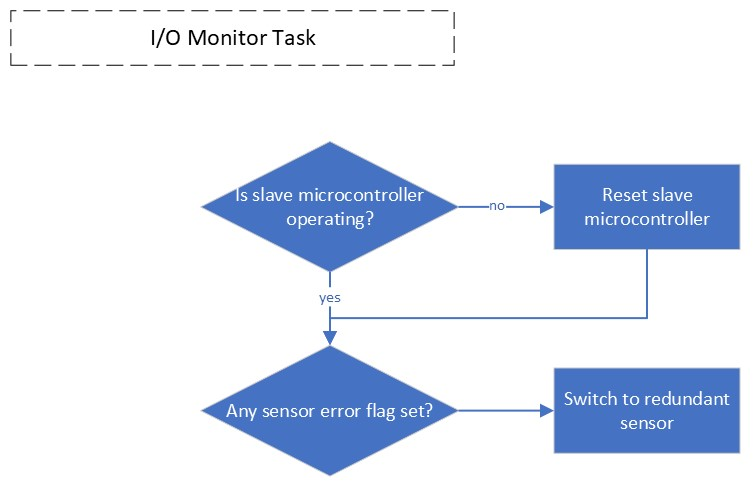
\includegraphics[width=0.65\textwidth]{./img/Section_4_2_2_4.jpeg}
  \end{center}
  \caption{I/O monitoring flowchart}\label{fig:flowchart-IO}
\end{figure}

The I/O Monitoring task is a low-priority task responsible for overseeing the status and functionality of the avionics system's input/output operations. Its primary function is to detect and manage potential errors or malfunctions in the sensors and the slave microcontroller. 

The task continuously checks if the slave microcontroller is operational. If the slave microcontroller is not responding, the I/O Monitor Task takes corrective action by resetting it to restore normal operation. Additionally, the task monitors error flags set by the sensor data capture tasks. If any sensor error is detected, the I/O Monitor Task initiates a switch to the redundant sensor. This process is detailed in the flowchart Figure~\ref{fig:flowchart-IO}.

\paragraph{LoRa Communications}
LoRa communications work is to be conducted by the ground stations team. However, this task is a lower priority task, responsible for transmitting data from the rocket to the ground station. It waits for a signal from the State Update and Event Logging task to begin transmission. 

Once triggered, it sends data packets over the LoRa link, including sensor data, state information, and event logs. This real-time data transmission allows for ground-based monitoring and analysis of the rocket's performance during flight. 

\paragraph{Memory Flashing}
\begin{figure}[ht!]
  \begin{center}
    \hspace{-1.5cm}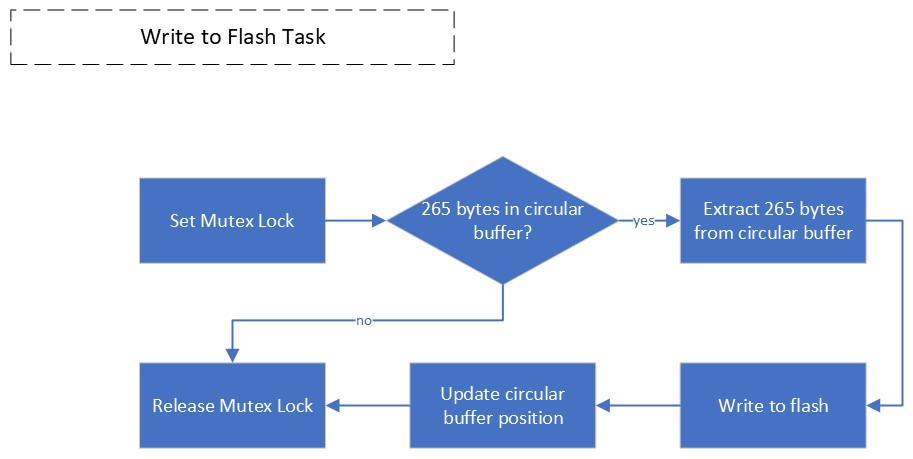
\includegraphics[width=0.75\textwidth]{./img/Section_4_2_2_5.jpeg}
  \end{center}
  \caption{Data storage flowchart}\label{fig:flowchart-flash}
\end{figure}

The Write to Flash Memory task (flowchart pictured Figure~\ref{fig:flowchart-flash}) is also low priority process that manages the storage of data frames in the onboard flash memory. It uses a mutex lock to ensure exclusive access to the flash memory, preventing conflicts with other tasks. The task checks if there are enough data frames in the circular buffer to fill a page (256 bytes). If so, it extracts the data frames from the buffer, writes them to flash memory, and updates the buffer position. This process is to repeat in the background unless a higher priority task requires the CPU time or until the flight ends.  

\subsection{Testing Plan}
\subsubsection{Verification}
\let\olditemize=\itemize \let\endolditemize=\enditemize \renewenvironment{itemize}{\olditemize \itemsep-0.5em}{\endolditemize}

\setlength\extrarowheight{-5em}
\begin{longtable}{<{\raggedright}p{4cm}p{10cm}}
\toprule Components & Test \\ \midrule
Accelerometer (High G) & Shake table:  
  \begin{itemize}
    \item Subject the accelerometer to known vibration profiles (frequencies, amplitudes from A1 data) 
    \item Verify output readings accurately reflect the applied vibrations.
  \end{itemize} \\
\midrule
Accelerometer (Low G) & Shake table:  
  \begin{itemize}
    \item Subject the accelerometer to known vibration profiles (frequencies, amplitudes from A1 data) 
    \item Verify output readings accurately reflect the applied vibrations. 
  \end{itemize} 
Saturation test:   
  \begin{itemize}
    \item Subject the accelerometer to vibration greater than the peak measurable by the sensor. 
    \item Observe the behaviour of the sensor after saturation – how long it remains saturated, accuracy of the data after leaving saturation.  
  \end{itemize}
 Tilt test:  
 \begin{itemize}
  \item Slowly rotate the accelerometer across its measurement axes.
 \end{itemize} \\
\midrule
Gyroscope & Rate table: 
  \begin{itemize}
    \item Mount gyroscope on a rate table that can rotate at different angular velocities. 
    \item Verify output accurately measures the applied rotation rates in each axis. 
  \end{itemize} 
Bias stability: 
  \begin{itemize}
    \item Leave gyroscope sampling data intermittently over a long period of time (overnight) 
    \item Measure average readings within a window of time at each interval, averaging the samples. 
    \item Measure resulting drift over time from initial values
  \end{itemize} \\
\midrule
Barometer & Vacuum chamber / temperature test:
  \begin{itemize}  
    \item Placing Barometer in a vacuum chamber and apply different pressure and temperature within a range relevant to expected flight altitudes.  
    \item Verify readings accurately reflect the known pressure values.
  \end{itemize} \\
\midrule
Magnetometer & Outdoor testing: 
  \begin{itemize} 
    \item Record data outdoors, with known changes in orientation. 
    \item Compare against expected magnetic field values for your location.
  \end{itemize} \\
\midrule
GPS & Outdoor testing: 
  \begin{itemize}
    \item Test in open locations under various conditions including stationary and while moving.  
    \item Evaluate accuracy against known locations or compare against high-precision reference GPS.
  \end{itemize} \\
\midrule
LoRa Communications & Transmission range: 
  \begin{itemize} 
    \item Test in different environments (clear line-of-sight and obstructed) to determine effective range.
  \end{itemize} 
 Data integrity:   
 \begin{itemize}
    \item Transmit known data packets and verify correct transmission.
  \end{itemize}\\
\midrule
 Flash Storage & Retention test:  
  \begin{itemize}
    \item Write data, power off for certain amount of time and verify data remains readable.  
\end{itemize} 
 Flash write timing: 
  \begin{itemize}
    \item Write different test data vectors to flash and measure the time it takes. 
    \item Perform tests with both full- and partial-page writes.
  \end{itemize}
 Flash read timing: 
  \begin{itemize}
    \item Read data back in from flash chip and measure the time it takes.
  \end{itemize} \\
\midrule
Microcontroller & Code execution test:  
  \begin{itemize}
    \item Test program functions. 
  \end{itemize} 
 Continuity test:  
 \begin{itemize}
  \item Monitoring signals and pin behaviour using logic analysers and oscilloscopes.
 \end{itemize}\\
 \bottomrule\\
 \caption{Proposed verification testing plan}\label{tbl:verification}
\end{longtable}

\subsubsection{Validation}
\setlength\extrarowheight{-5em}
\begin{longtable}{<{\raggedright}p{4cm}p{10cm}}
\toprule
Sub-Assemblies &
  Test \\
\midrule
Recovery Assembly (Sensors, Mirco and GPS) & Data injection tests 
  \begin{itemize}
    \item Place system in a testing mode, connecting recovery outputs to some readable output (i.e. buzzer, LED). 
    \item Feed in data collected from previous flights and determine if recovery system “fires” at the known apogee.
  \end{itemize} \\
\midrule
Gound Communications & Telemetry reception:  
  \begin{itemize}
    \item Test reception of data from Avionics Bay, ensuring that data is correctly being transmitted.
  \end{itemize} \\
\midrule
Storage & Data logging:  
  \begin{itemize} 
    \item Validate that sensor data is correctly being stored in flash.
  \end{itemize} \\
\midrule
Internal Communications (CAN bus) & Message integrity 
  \begin{itemize}
    \item Test transmission and reception of all expected message types over the CAN bus.
  \end{itemize} \\
\midrule
State Estimation & Simulation:  
\begin{itemize}
  \item Use a simulator to input realistic sensor data. Verify state estimation algorithms correctly calculate state estimation.
\end{itemize} \\
\midrule
SRAD Redundancy & Error injected testing:  
\begin{itemize}
  \item Testing for failover between primary and secondary systems.  
  \item Place system in a testing mode, inject errata on communication lines (payload/aerobrakes CAN, SPI, etc.) 
  \item Verify system correctly identifies sources of error and appropriately swaps to redundant system.
\end{itemize} \\\bottomrule\\
\caption{Proposed validation testing plan}\label{tbl:validations}
\end{longtable}

\subsubsection{Operation}
Prior to launch, a final ground test will be conducted using flight-like sensor data taken from A1 and A2 profiles. This test will run the Avionics system in "test mode" where simulated packets are transmitted, successful SRAD deployment is indicated through an LED, and aerobrake deployment is verified. This final check verifies correct data flow, decision-making logic, and functionality of both the recovery and aerobrakes systems. 


\subsection{Data Processing and Analysis}
Development of data processing tools and algorithms was in large part a significant challenge within the progression of the project. These systems were developed offline first, mostly through the implementation of scripts built with Python, through analysis of the data that was collected after the flight of Aurora I. 

This section outlines these systems as they were designed, and how they were and will continue to be applied for the analysis of data throughout future Aurora rockets.

\subsubsection{Attitude Estimation}
As touched on previously, it is important that the rocket maintains some representation of its orientation relative to a global frame of reference during the flight. Since the accelerometers included within the available sensor suite are only able to perform inertial measurement relative to the body axis of the vehicle, the rotational information is applied to rotate and scale these values to determine a true vertical acceleration to apply in further calculations.

The instantaneous angular rate measurements output by the gyroscopic sensors can be considered as time derivatives of the Euler angle representation of the rocket's attitude. As such, by constructing rotation quaternions from these instantaneous rates and applying the rotation to the previously determined attitude (simply the last calculated rotation quaternion), effectively a numerical integration process is applied:\\[0.5em]
{
\setlength{\belowdisplayskip}{5pt}%
\setlength{\abovedisplayskip}{-15pt}%
\begin{align*}
  \intertext{First the angular rates in $\unit{\degree}/\unit{\second}$ are converted to Euler angles (radians):}\\
  \begin{bmatrix}
    \phi\\\theta\\\psi
    \end{bmatrix} &= \frac{\pi}{180}\cdot\begin{bmatrix}
                                        \omega_x\\\omega_y\\\omega_z
                                        \end{bmatrix}\\
    \intertext{A unit quaternion is then initialised through the half Euler angles (per equation 66 ~\cite{Diebel2006})}\\
    \dot q &= 
    \begin{bmatrix}
      c_{\phi/2}c_{\theta/2}c_{\psi/2}-s_{\phi/2}c_{\theta/2}s_{\psi/2}\\
      c_{\phi/2}c_{\theta/2}c_{\psi/2}+s_{\phi/2}s_{\theta/2}s_{\psi/2}\\
      c_{\phi/2}s_{\theta/2}s_{\psi/2}-s_{\phi/2}c_{\theta/2}s_{\psi/2}\\
      c_{\phi/2}c_{\theta/2}s_{\psi/2}+c_{\phi/2}c_{\theta/2}s_{\psi/2}\\
    \end{bmatrix}\\[0.5ex]
    \intertext{Where $c_x=\cos{x}$, $s_x=\sin{x}$. Then from equation 102~\cite{Diebel2006}:}\\
    q_{k} &= q_{k-1}\cdot\dot q\\
          &= \begin{bmatrix}
            (q_{{k-1}_0}  \dot q_0) + (-q_{{k-1}_1}  \dot q_1) + (-q_{{k-1}_2}  \dot q_2) + (-q_{{k-1}_3}  \dot q_3)\\
            (q_{{k-1}_0}  \dot q_1) + (q_{{k-1}_1}  \dot q_0) + (q_{{k-1}_2}  \dot q_3) + (-q_{{k-1}_3}  \dot q_2)\\
            (q_{{k-1}_0}  \dot q_2) + (-q_{{k-1}_1}  \dot q_3) + (q_{{k-1}_2}  \dot q_0) + (q_{{k-1}_3}  \dot q_1)\\
            (q_{{k-1}_0}  \dot q_3) + (q_{{k-1}_1}  \dot q_2) + (-q_{{k-1}_2}  \dot q_1) + (q_{{k-1}_3}  \dot q_0)
             \end{bmatrix}\\
    \intertext{Finally, normalise the quaternion to $[-1,1]$:}\\
    q_{normal} &= q_{k} / \sqrt{q_{k_0}^2 + q_{k_1}^2 + q_{k_2}^2 + q_{k_3}^2}
\end{align*}
}\\

\noindent The resulting quaternion as calculated through the integration of angular velocities then represents the rotation of the rocket body from its initial pose.

\subsubsection{State Estimation (Velocity and Altitude)}
In order to determine information on the rocket's displacement and upward velocity, a Kalman Filter is applied for greater accuracy in estimation. The filter operates in two steps, first predicting future state values and then updating the predictions through measurement and calculated errors.

\citetitle{Welch1995} describes the following equations for a linear Kalman filter:\vspace{-3em}

\begin{align*}
    &\intertext{Time update (predict):}
    &\text{(1) Project the state ahead} \\
    &\hat{x}_k^- = A \hat{x}_{k-1} + B u_{k-1} \\[0.5em]
    &\text{(2) Project the error covariance ahead} \\
    &\bar{P}_k = A P_{k-1} A^T + Q\\
    &\intertext{Measurement update (correct):}
    &\text{(1)& Compute the Kalman gain} \\
    &K_k = \bar{P}_k H^T (H \bar{P}_k H^T + R)^{-1} \\[0.5em]
    &\text{(2) Update estimate with measurement } z_k \\
    &\hat{x}_k = \hat{x}_k^- + K_k (z_k - H \hat{x}_k^-) \\[0.5em]
    &\text{(3) Update the error covariance} \\
    &P_k = (I - K_k H) \bar{P}_k
\end{align*}\\

The state is defined as a tri-cell column vector $x = [s, v, a]^T$ for the rocket's altitude, upward velocity, and upward acceleration. The system is modelled with constant acceleration, where $v$ and $s$ are simply integrated from $a$. This results in a state transition matrix $A$:
\addcontentsline{equ}{chapter}{Kalman Filter}
\begin{equation}
  A = \begin{bmatrix}
        1& dt& \frac{1}{2}dt^2\\
        0& 1& dt              \\
        0& 0& 1
      \end{bmatrix} 
  \label{eq:kalmanA}
\end{equation}
\myequation{State transition model $A$}

Since $s$ and $a$ are measured directly through the barometer and accelerometer respectively, the corresponding measurement model is then:

\begin{equation}
  H = \begin{bmatrix}
        1 & 0 & 0\\
        0 & 0 & 1
      \end{bmatrix}
  \label{eq:kalmanH}
\end{equation}
\myequation{Measurement model $H$}

Assuming no control input to the system, $B$ and $u$ are both omitted. The measurement of $s$ is simply the altitude as calculated directly from the barometric data, while $a$ must be processed as part of the measurement update.

As the measured acceleration is in reference to the rocket's body axis, the tilt angle is applied to compensate. The previously determined attitude quaternion rotates a unit vector $\uvec{z}$, representing the global vertical axis, to the rocket's body frame axis $\bm{\hat{\textbf{z}}_B}$. The dot product of these two vectors provides the cosine of the tilt angle $\cos{\theta} = \bm{\hat{\textbf{z}}_B}\cdot \uvec{z}$, which is multiplied by the measured acceleration to determine the upwards acceleration in the global frame of reference. 

Given the inertial measurement of the accelerometer includes the reactionary force opposing acceleration due to gravity, this must also be subtracted from the measurement in order to purely determine the upward acceleration of the rocket. The resulting measurement vector follows:
\begin{equation}
  z = \begin{bmatrix}
        s\\
        (\cos{\theta}\cdot a)-g
      \end{bmatrix}
  \label{eq:kalmanZ}
\end{equation}
\myequation{Measurement $z$}

Fortunately, the Blue Raven flight computers provide flight data post-recovery against which the performance of these calculations can be measured. A particular advantage of this is that it provides greater flexibility in tuning the noise parameters $Q$ and $R$ of the filter. These were determined offline through a technique provided by the \textit{BayesianOptimization}~\cite{Bayesian2014} Python module. 

The routine calculating state with the implemented filter was fed into the optimisation module, returning a root mean square error between the calculated estimate and the measurements from the Blue Raven. Over several iterations this then determines the noise parameters corresponding to best performance, which can then be applied within the filter.

\section{Aurora I Results and Analysis}
Following the successful launch of Aurora I, data was collected by reading serial output from the onboard flash, processing the dataframes specified in Section~\ref{sec:dataframe} into CSV data for offline handling. 

Appendix~\ref{apdx:B} provides graphs of the resulting raw data for high resolution accelerometer and gyroscope data, plotted against the corresponding output provided by the Blue Raven. Unfortunately, due to a configuration error barometric data was found irretrievable during this process, however the data provided by the Blue Raven was able to be used as a backup for processing in calculations where necessary.

As the graphs indicate, the avionics system largely provided satisfactory results compared to the Blue Raven's collected data. Some artifacts are noticeable, likely due to the sourced components being last minute backups, however the hope was that the previously discussed processes would largely eliminate the resulting noise. 

\begin{figure}[ht!]
  \begin{minipage}{0.5\textwidth}
    \includegraphics[width=\textwidth]{./img/plot/state/attitude/quat_AV.png}
  \end{minipage}
  \begin{minipage}{0.5\textwidth}
    \includegraphics[width=\textwidth]{./img/plot/state/attitude/quat_BR.png}
  \end{minipage}
\caption{Comparison of quaternion estimates}\label{fig:quat-estimates}
\end{figure}

Figure~\ref{fig:quat-estimates} outlines a comparison of the estimated attitude quaternions for the first fourteen seconds of flight. Apogee of the rocket occurred at approximately $t=\SI{10.3}{\second}$, and it is apparent in these graphs that the attitude as estimated by the avionics system is largely equivalent to that of the Blue Raven to that point. There is some small deviation in scaling on the $x$ and $y$ components, however this error is within an acceptable margin for the flight. More data is required before it can be determined that these results are satisfactory for the processes to be applied for the Aurora V launch, however at present it appears promising.

Post-apogee the error margin widens, as becomes most apparent from $t=\SI{12}{\second}$ to $t=\SI{16}{\second}$. This is most likely a result of the rocket's orientation rapidly oscillating as a result of the recovery deployment, accentuating the gyroscopic drift. It is also possible that the shock from the detonation charges used during deployment could have damaged the sensors, so further data is required and it is intended that this will be analysed through pop tests.

The resulting velocity calculated by the designed Kalman Filter is provided in Figure~\ref{fig:kalman}. This graph highlights the two recovery deployment events for the drogue and main chutes. For the best accuracy, the filter is treated as operating within the three discrete regions that are isolated by these events; These regions will be referred to as regions $A$, $D$, and $M$ for ascent, drogue, and main respectively.

\begin{figure}[ht!]
  \centering
  \includegraphics[width=0.65\textwidth]{./img/plot/state/Velocity_X.png}
  \caption{Comparison of quaternion estimates}\label{fig:kalman}
\end{figure}

Within each of these regions, the noise parameters $Q$ and $R$ were recalculated in isolation through the described Bayesian Optimisation. This allows for the filter to provide a better estimate according to the change in conditions. As indicated by the plot, the model performs ideally through the entirety of region $A$. This region is most important to the application of the filter as only the values that it bounds will be delivered to the subsystems requiring these metrics. 

At present the filter struggles to accurately predict the velocity in regions $D$ and $M$. Solutions to this issue are currently being explored, however current best assumptions lean towards an insufficient model (Equation~\ref{eq:kalmanA}) being employed. Due to the limited necessity of accuracy within these regions, realistically only providing better visualisation for the ground station following recovery deployment, development of a solution is currently allocated as a low priority.

\subsection{Key Findings and Next Steps}
Through the data retrieved from the flight of Aurora I, initial findings were surprisingly positive with respect to the understanding that less than ideal hardware was employed. Raw data was correctly sampled, with the exception of barometric information, and was easily retrievable through associated dataframes. Analysis tools and data processing implementations also performed admirably.

Current points of interest surround the performance of these same tools and algorithms with data gathered from the launch of Aurora II, where ideally performance metrics should remain similarly impressive. Following this, Aurora III and onwards will be particularly important with the move to custom hardware and an ideally better performing and more robust sensor suite.

\section{Project Management and Timeline}
Table~\ref{tbl:timeline} outlines the timeline of all Aurora rocket launch dates. These dates will serve as guide for when software and integration tests are to be completed. Due to the tight timeline between launch dates, coordination with other subsystems must be organised to ensure that data analytics and verification process can be put in place and tested. The nature of this capstone project is depended on the implementation of subsystems, primarily Avionics hardware and Aerobrake mechanisms.  

At the point when this report is submitted, the next launch will be on the 15th of June.  With the launch in two weeks, the aim is to implement a basic version of the Real-Time Operating System (RTOS) by Aurora IIIb, if not by IIIa. Aurora III will involve the implementation of our final design for Aurora IV. The Aurora IIIb launch will serve as an opportunity to make necessary corrections, primarily through the collection of additional data. Final designs and implementations are expected to be completed by Aurora IV.  

The timeline is subject to potential adjustments based on the progress of hardware verification and testing, as well as any unforeseen challenges that may arise during development. The team remains committed to meeting the deadlines and ensuring the timely completion of the project. 

\setlength\extrarowheight{1em}
\begin{table}[h]
\centering
\begin{tabularx}{\textwidth}{XllX}
\toprule
\textbf{Milestone} & \textbf{Date Completed} & \textbf{Status} & \textbf{Notes} \\
\midrule
Aurora I Launch & 14-04-2024 & Completed & Successful data collection, preliminary analysis completed. \\
Aurora II Launch & 05-05-2024 & Completed & Additional barometer data collected, no major design changes from Aurora I. \\
Aurora IIIa \& IIIb Hardware Verification \& Testing & 15-06-2024 & In Progress & Ongoing verification and validation of new hardware components, integration with RTOS, and refinement of sensor fusion and state estimation algorithms. \\
Aurora IV Launch & 27-07-2024 & Pending & Full-system integration test, flight test to validate real-time data transmission and overall system performance. \\
Aurora V Launch (AURC Competition) & 20-09-2024 & Pending & Final flight test, incorporating all refinements and optimisations based on data and feedback from previous launches. Competition readiness assessment and final report. \\
\bottomrule
\end{tabularx}
\caption{Full project timeline with respect to launch deadlines}\label{tbl:timeline}
\end{table}

\subsection{Risk Assessment and Mitigation}
Although the most risks were outlined in our proposal and risk assessment, it is worth noting that there will additional risk primarily from conducting verification and validation of hardware. To validate the avionics senor suite, a range of tools will be required which include, shake tables, vacuum chambers and rate tables. Such tools will be accessed through RMIT physics department and laboratory. 

Currently, the team is working closely with technical officer Peter McGlynn to assist with providing access to the relevant tools. Although most tests will be relatively straight forward, the use of a vacuum chamber to test the barometer poses a safety concern. In addition to controlling a vacuum, it is planned to have a heat source to within the chamber to adjust the temperature, simulating the temperate increase in the rocket’s environment during flight. 

It was suggested that toaster wires can be fed through the camber to do so. Creating and using such mechanism will be challenging, however all activity and equipment risk assessments will be completed before any validation testing is conducted.  

\section{Discussion and Recommendations}

\subsection{Critical Evaluation of Progress}
The project is progressing well towards meeting its objectives and deliverables. The successful launch of Aurora I and the resulting data analysis have provided valuable insights into the performance of the avionics system and identified areas for improvement. The implementation of the RTOS in Aurora III will significantly enhance the system's ability to handle complex tasks and meet real-time requirements. 

The data collection and logging processes are functioning as intended, and the initial validation tests have shown promising results. However, there are areas that require further attention. Although the RTOS implementation is feasible, this is the first time any team member has used an RTOS. Extensive testing and validation are required, ensuring that software design is operating in a flight environment as intended. 

Additionally, the integration of the avionics system with the aerobrakes and payload subsystems also requires thorough testing and validation to ensuring aerobrake processes are triggered at the right time.  

\subsection{Future Recommendations}
The tight deadlines associated with rocket launches highlight the need for a more proactive approach to testing and validation. A more detailed plan is required, outlining how and when testing of both individual components and integrated subsystems is to be completed, which includes ground tests and simulations to identify and address potential issues before the rocket takes flight. 

Furthermore, the delays in hardware highlight the importance of utilising simulation environments as testing platforms during waiting periods. Although some simulation was conducted, it is recommended to priorities tests, especially when using new techniques such as RTOS and real-time data processing.  

\section{Conclusions}
The Data Analytics and Verification project has made significant progress in developing a custom data analytical software for the Aurora V rocket. The successful launch of Aurora I and the resulting data analysis have provided valuable insights for refining the system's design and algorithms. The implementation of a Real-Time Operating System (RTOS) in Aurora III represents a major advancement in the system's architecture, enabling efficient task management and real-time responsiveness. 

While challenges still remain, such as the need for extensive testing and validation of the RTOS and further refinement of sensor fusion and state estimation algorithms, the project is on track to deliver a competition-ready solution for Aurora V. The team's proactive approach to risk mitigation and the iterative development process will ensure that the final system is capable of meeting the strict requirements of the AURC competition with the aim of scoring high from data analytical perspective. 

The knowledge and experience gained through this project will not only contribute to the success of Aurora V but also have broader implications for the field of data analytics and verification in aerospace applications. By implementing real-time data analysis in resource-constrained environments, findings through this capstone can act as a resource for future competition RMIT model rockets.  


  \bibliographystyle{ieeetr}
  \printbibliography

  \renewcommand{\thechapter}{\Alph{chapter}}
\renewcommand{\thefigure}{\Alph{chapter}.\arabic{figure}}
\renewcommand{\chaptername}{Appendix}
\addcontentsline{toc}{part}{Appendix}

\clearpage
\chapter{}\label{apdx:}
\setlrmarginsandblock{0.5cm}{0.5cm}{*}
\checkandfixthelayout
\vfill{}
\vfill{}

\end{document}
